% ------ headers globales y begin ---------------
\documentclass[11pt, a4paper, twoside]{article}
\usepackage{header_tp2}
\begin{document}{}
% -----------------------------------------------
\begin{comment}
\begin{figure}[H]\begin{center}
\begin{tikzpicture}[decoration=penciline, decorate]
  \draw[decorate,style=help lines] (-2,-2) grid[step=1cm] (4,4);
  \draw[decorate,thick] (0,0) -- (0,3) -- (3,3);
  \draw[decorate,ultra thick,blue] (3,3) arc (0:-90:2cm);
        % supposed to be an arc
  \draw[decorate,thick,pattern=north east lines] (-0.4cm,-0.8cm)
    rectangle (1.2,-2);
  \node[decorate,draw,inner sep=0.5cm,fill=yellow,circle] (a) at (2,0) {};
        % That's not even an ellipse
  \node[decorate,draw,inner sep=0.3cm,fill=red] (b) at (2,-2) {};
  \draw[decorate] (b) to[in=-45,out=45] (a);
        % This was supposed to be an edge
  \node[decorate,draw,minimum height=2cm,minimum width=1cm] (c) at (-1.5,0) {};
  \draw[decorate,-,dashed] (-0.5cm,-0.5cm) -- (-0.5cm,3.5cm)  -| (c.north);
\end{tikzpicture}
\end{center}\caption{Tiempo en función del radio}\end{figure}

\begin{center}\fixme{}\end{center}
\end{comment}

Lo primero que hicimos fue contrastar nuestro cálculo teórico de la complejidad con una medición empírica de los tiempos de ejecución. Utilizamos entradas generadas aleatoriamente, con distintos tamaños de tablero. 


\begin{figure}[H]
   \begin{center}
   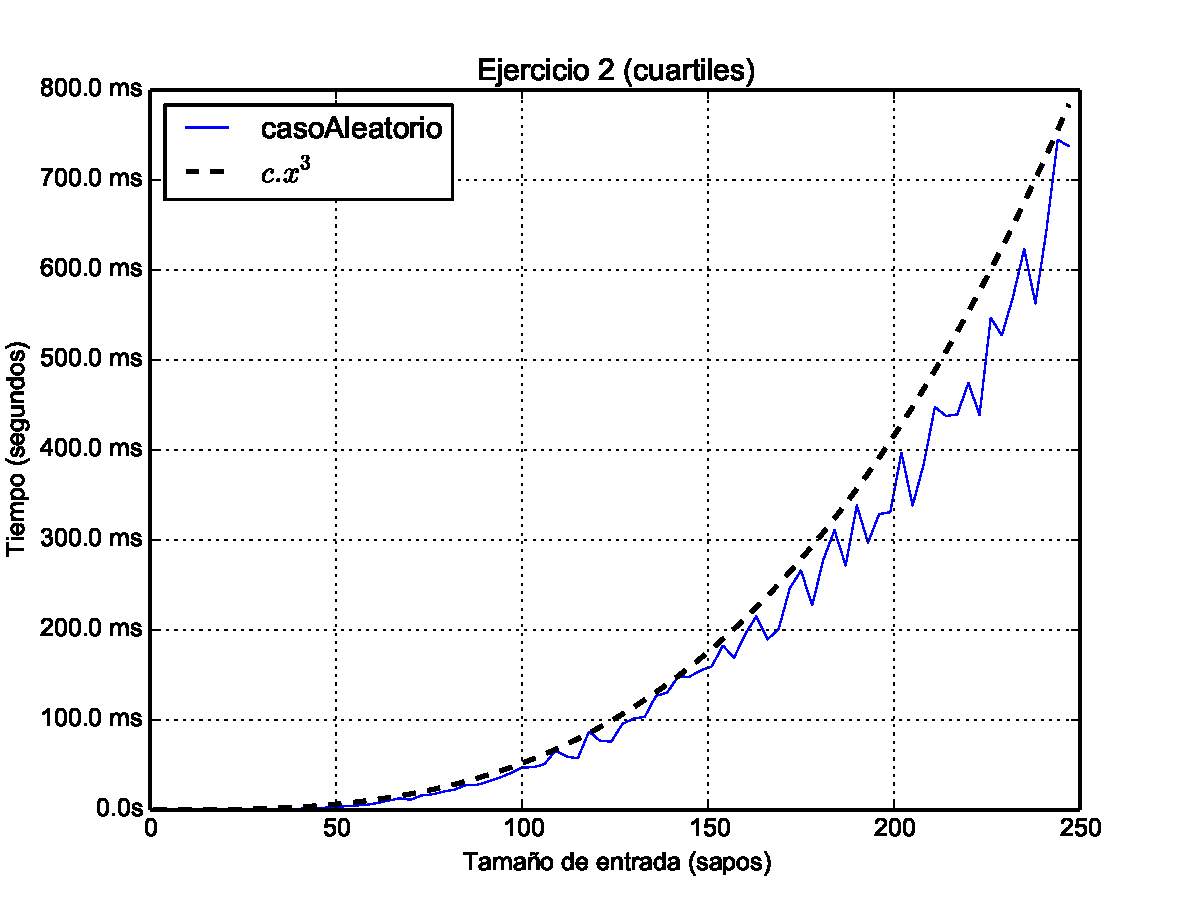
\includegraphics[width=1.4\textwidth,angle=90]{../ej3/graficos/test_tiempoLiso.pdf}
   \caption{\textbf{Tiempo de ejecución en función de la cantidad de centrales ``ITA'' de gas.}}
   \label{fig:ej3-graf-1}
   \end{center}
\end{figure}
\clearpage


%Observamos una curva que crece bastante rápido. Para corroborar que la complejidad es \bigO{n^3*k}, graficamos el cociente entre el tiempo de ejecución y la función $f(x)$ = $x^3$. Se puede ver al cociente estabilizándose acerca de una constante, lo que nos permite aventurar a decir que el algoritmo cumple con su cota propuesta.

Realizamos una tercer medición más interesante. Intuitivamente, nos dimos cuenta de que si el casillero de origen y el de destino están cerca, el algoritmo iba a encontrar el camino más rápidamente. Esta noción de cercanía no es solo la proximidad de los casilleros de la matriz. Es mucho más interesante. Depende de como están distribuidos los resortes de distintas potencias, y, claro, de las unidades extras con que cuente. Se nos ocurrió fijar un tamaño de entrada y generar matrices con distintos valores de potencia y distintos valores de potencia extra. Luego hicimos correr el algoritmo, guardando tanto su tiempo de ejecución como su resultado, es decir, la cantidad mínima de saltos para llegar a destino. Ordenamos de acuerdo al resultado y podemos ver una correlación positiva entre el resultado y el tiempo de ejecución. 

\begin{figure}[H]
   \begin{center}
   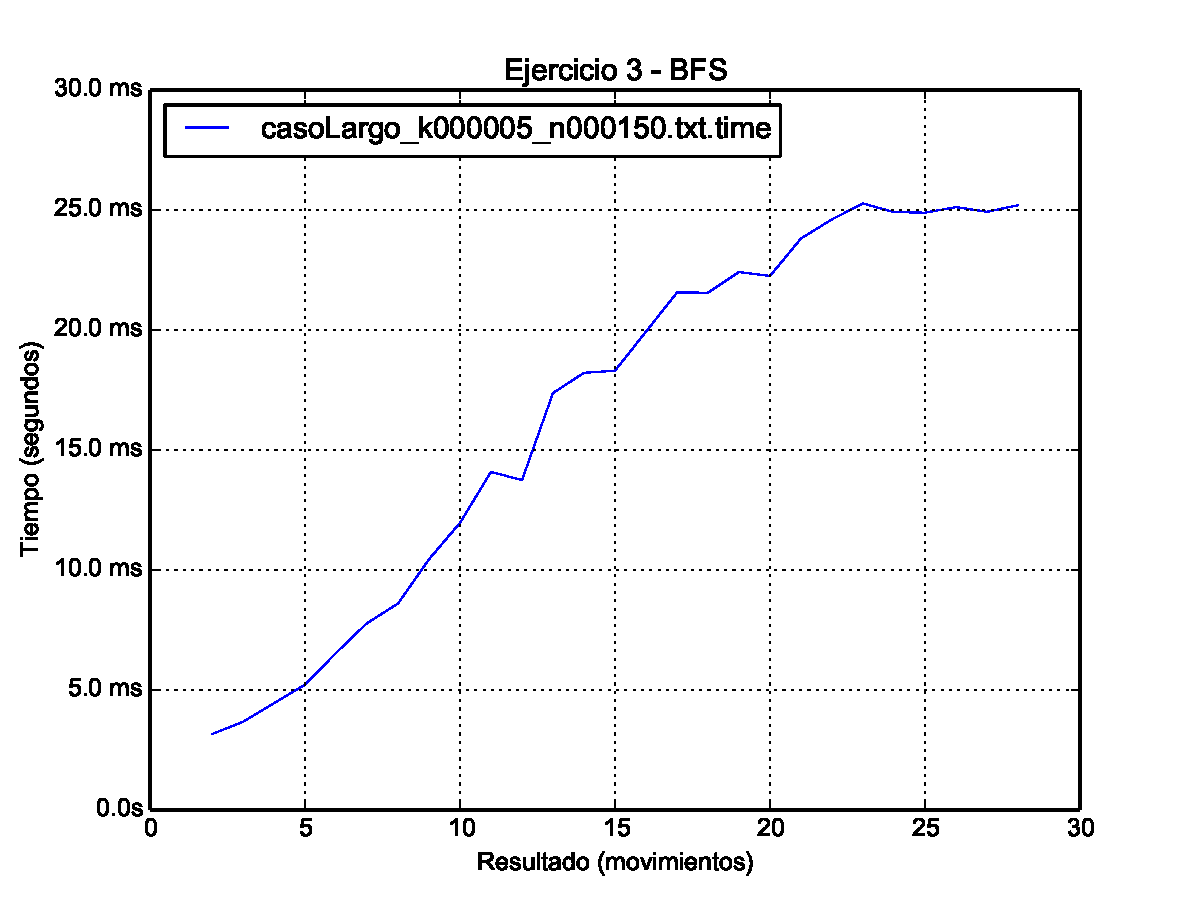
\includegraphics[width=1.4\textwidth,angle=90]{../ej3/graficos/test_porTamanhoSalisa.pdf}
   \caption{\textbf{Tiempo de ejecución en función de la cantidad de centrales ``ITA'' de gas.}}
   \label{fig:ej3-graf-1}
   \end{center}
\end{figure}
\clearpage

Por último, el tiempo del algorítmo también depende del tamaño de ``k''. Es decir, cuanto mas grande es la cantidad potenciadores del caso a analizar mas cantidad de cálculo hay que realizar. Esto se puede visualizar en el siguiente gráfico:


\begin{figure}[H]
   \begin{center}
   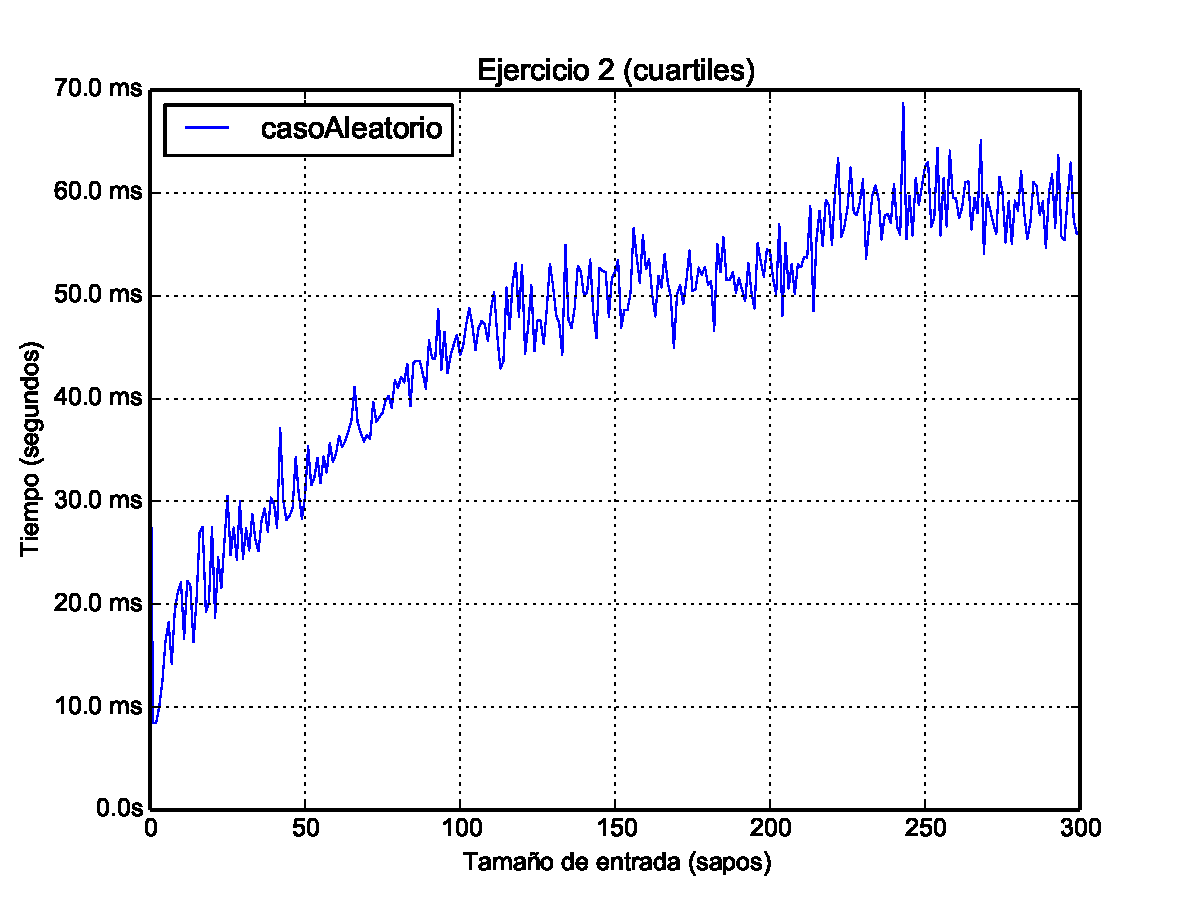
\includegraphics[width=1.4\textwidth,angle=90]{../ej3/graficos/test_potExtra.pdf}
   \caption{\textbf{Tiempo de ejecución en función de la cantidad de centrales ``ITA'' de gas.}}
   \label{fig:ej3-graf-1}
   \end{center}
\end{figure}
\clearpage

\end{document}
% -----------------------------------------------
